\documentclass[12pt]{article}
\usepackage[utf8]{inputenc}
\usepackage{float}

\textwidth 15cm \oddsidemargin 1cm \topmargin -0.5cm \textheight 22cm \footskip 1.5cm 
% \usepackage{epsfig}

    
\usepackage{longtable}
\usepackage{supertabular}
\usepackage{hyperref}%pdf段落链接
\usepackage{natbib}%references
\usepackage{graphicx}%photos
\usepackage{indentfirst} %首行缩进
\usepackage{fancyhdr}%页眉页脚等
\usepackage{multirow}%表格的强制换行
\usepackage{verbatim}%多行注释
\usepackage[table,xcdraw]{xcolor}
\usepackage{caption}
\usepackage{graphicx, subfig}
% \usepackage{biblatex}
% \addbibresource{references.bib}
\usepackage{natbib}
% \graphicspath{{/Users/xiaozhan/Documents/groupproject}}

\def\n{\noindent}

\pagestyle{plain}
\pagestyle{fancy}%logo
\rfoot{
\includegraphics[scale=0.21]{kcl.png}} 
\cfoot{\thepage} 

\lhead{King's College London}
\renewcommand{\headrulewidth}{0.5pt}

\begin{titlepage}
\title{\Huge $\mathbf{7CCSMGPR: 
Final \; Report}$}
\author{\Large \textbf{Group Name: Keep Trying} }
\date{10/03/2019}
\end{titlepage}


\begin{document}
\maketitle

\begin{flushright}
\vspace{3cm}

\large \begin{tabular}{ll}
Members:&\\
1816772 & Dongang Ji \\
1844334 & Xiao Zhan \\
1805051 & Xiaoxue Bai\\
1822709 & Xiaoyue Peng\\
1842973 & Ying Yu\\
1804098 & Yingdi Song\\
\end{tabular}
 
\end{flushright}

\thispagestyle{empty}

\newpage
\tableofcontents



\thispagestyle{empty}




\newpage
\setcounter{page}{1}
\vspace{5cm}


\section{Introduction}
%我们小组的任务是实现一个multi-host file synchroniser 。这个multi-host file synchroniser中有一个手机客户端和网页客户端(one for desktop,one for mobile),将它俩局域网连接起来,通过服务器上连接到一个数据库,在数据库中存储使用这个multi-host file synchronise的所有用户信息和其中的文件信息。ios mobile client 和 desktop client 


\noindent The task of our team is to implement a multi-host file synchroniser. A multi-host file synchroniser usually comprises of a mobile client and a desktop client which are connected through LANs. By connecting to a database through the server, and storing the multi-host in the database which contains all user information and its file information, our multi-host file synchroniser is able to achieve functionalities as follows.

%最后达成的整体功能为:
%首先用户可以在desktop client和mobile client进行注册然后登陆进入软件,用户的密码会用MD5加密算法加密后存储到数据库中。登陆成功后首先进入的是主菜单界面,主菜单界面显示该登陆用户有权限查看和修改的文件的文件列表,同时也显示了每个文件的最后修改时间和修改用户。用户同时可以在这个界面进行上传和创建文件。点击具体文件会进入到这个文件的文件界面,用户可以在这个界面进行修改和上传。同时,文件的创建者即为这个文件的管理者,可以对其他用户的权限进行管理,包括查看权限和修改权限,也可以删除特定用户的修改权限。除此之外还有用户界面,可以在编辑用户的资料和修改密码。


\vspace{0.2cm}
\noindent First, the user can register with the desktop client and the mobile client, and log in to the software. The user's password is encrypted by the MD5 encryption algorithm and is stored in the database. After the successful login, the main menu interface is entered. The main menu interface displays the file list which contains the files that the login user has permission to view and modify, and also displays the last modification time of each file and the modified user. Users can also upload and create files in this interface. Clicking on a specific file will take you to the file interface of this file, and the user can modify and upload it through this interface. At the same time, the creator of the file is the administrator of the file, which can manage the permissions of other users, including viewing permissions and modifying permissions, and also deleting the modification permissions of specific users.In addition to this there is a user interface where you can edit the information of user and change the password.

%-desktop
%desktop端我们制作了一个web,在 Macintosh Apache MySQL PHP 平台下使用php进行开发。Macintosh Apache MySQL PHP 专门用来在 Mac 环境下搭建 Apache、MySQL、PHP 平台。主要使用的是为简化企业级应用开发和敏捷WEB应用开发而诞生的thinkphp框架。
 
%-ios
%Mobile端我们制作了一个ios软件,使用swift5在xcode软件中进行开发,利用基于Swift 的HTTP 网络库—Alamofire网络开发框架实现核心功能,演示时我们将使用模拟器展示软件效果。

%在代码实现时,我们使用MVC设计模式,将程序的输入、处理、和输出分开,增强了代码美学,使代码更加灵活,重用性更高

% main problems

%每个文件在创建的时候,数据库中会存有他们的版本号,原始文件的版本号为0,每修改一次上传后,版本号加1,在点进这个文件的具体页面的时候,会显示这个文件的所有版本。如果有两个用户同时修改上传文件的时候,解决的办法为:假设两个用户A、B打开的文件版本号都为0,然后用户A先修改完成进行上传,这个时候系统会检测用户A打开的文件版本号是否和这个文件的最新版本号一致,如果这个文件的最新版本号依然为0,则用户A上传成功,版本号为1。这个时候用户B再修改上传,系统检测到用户B打开的文件版本号为0,而最新的版本号为1,系统则在页面显示最新版本号的文件内容,即为A的修改后上传的文件内容,B进行阅读参考后决定是否上传,假设B决定上传自己修改后的文件,则B上传的文件版本号为2。

\vspace{0.2cm}
\noindent When each file is created, the version number of the original file will be stored in the database. The version number of the original file is 0. After each modification, the version number is increased by 1. When you click into the specific page of this file, all versions of this file will be displayed. If two users modify the uploaded file at the same time, the solution is as follows: Assuming that the version number of the file opened by the two users, A and B, is 0, and then the user A first completes the modification and uploads. At this time, the system detects whether the file version user A opened is consistent with the latest version number of this file. If the latest version number of this file is still 0, user A uploads successfully and the version number is 1. Then user B finishes the change and uploads his file. The system detects that the version number of the file opened by user B is 0, but the latest version number is 1, then the system displays the file content of the latest version number on the page, that is, the content of  the file uploaded after the modification of user A. Then user B decides whether to upload after reading the contents. Assuming that B still decides to upload the modified file, the version number of the file uploaded by user B is 2.

%multi-host file synchroniser we made 把文件上传到服务器上,不占用电脑空间,只有在有网络的情况下才可以进行操作。同时这个synchroniser保证文件的隐秘性,文件创建者为这个文件管理者,自已自主选择给哪个用户查看权限和修改权限。当前市面上有很多类似的平台可以实现这些功能,例如Google drive和dropbox,相比较已上市的平台,虽然成熟度上相比我们还是有很大的不足,但是我们synchroniser的优点在于系统自身的高度自主性,在出现同步上传矛盾的时候,不依赖于一些特定的系统规则,而是把同步上传的版本显示给用户进行选择,这样既不违反时间顺序原则,也人为的避免了关于文件内容的矛盾。我们的project由于资源、资金、时间和技术的限制,导致没有做出一个非常成熟可以直接让大众使用的软件,但是我们小组对文件同步云端的未来非常看好,可以也希望在以后的工作能有机会再次接触这个方面,弥补当前软件的不足做出更好的软件。
\vspace{0.2cm}
\noindent The multi-host file synchroniser we made uploads files to the database without taking up computer storage space when there is a network. At the same time, the synchroniser guarantees the confidentiality of the file. The file creator is the file manager, and the manager can choose which user to own the view permission and the modification permission. There are many similar platforms on the market that can implement these functions, such as Google drive and dropbox. Compared with the platform already listed, although we still have a lot of shortcomings in maturity, the advantage of our synchroniser is the high autonomy of the system itself. In the case of synchronous upload conflicts, it does not depend on some specific system rules, but displays the synchronously uploaded version to the user for selection, which does not violate the chronological principle, and artificially avoids the content of the file contradiction. Due to limitations in resources, funding, time and technology, our project did not make a very mature software that can be directly used by the public, but our team is very optimistic about the future of the file synchronization cloud, and we hope that we can have a future work opportunity to reach out to this aspect again, make up for the lack of current software to make better software.

\noindent The rest of the report is structured as follows. In Section \ref{Sec:Sec2}




\section{Review}
\label{Sec:Sec2}
\noindent A cloud synchronization("sync")application synchronizes data hosted by a cloud storage service(e.g.,Dropbox,Google Drive,Microsoft Google Drive,etc.) For example,Dropbox announced that it has hit a new milestone of 300 million users, adding 100 million users in just six months.\citep{7417235}

\vspace{0.2cm}
\noindent Multi-user collaboration and synchronization are nowadays essential features in cloud storage services.\citep{MOSCICKI20181052}Ideally, this kind of cloud storage can provide users with a convenient environment.In file sharing scenario, 


\vspace{0.2cm}
\noindent At present, several applications and platforms that have been successfully implemented on the market have Google Drive, Dropbox, etc., but Google Drive is more comprehensive and richer than Dropbox. Specifically, Google Drive has sophisticated and powerful sharing capabilities, and enables online editing and support for documents in different formats.

\begin{comment}
Jakub T. Mo艣cicki, Luca Mascetti,
Cloud storage services for file synchronization and sharing in science, education and research,
Future Generation Computer Systems,
Volume 78, Part 3,
2018,
Pages 1052-1054,
ISSN 0167-739X,
https://doi.org/10.1016/j.future.2017.09.019.
\end{comment}

\vspace{0.2cm}
\noindent With the collaboration feature, no matter where the participants are, whether the user is using the mobile phone or the web page, he or she can write a document together with teammates, just like sitting together to discuss. Users can see other all editorial behaviors of everyone, and can be commented or discussed in real time, this is an efficient way of working, and also the main function our group project want to achieve.

\vspace{0.2cm}
\noindent Mobile devices have changed how we conceive software. There is a great range of development alternatives.At present, mobile web applications have been widely used, and there are many examples and valuable experiences in the current development background and field.\citep{7128878}


%Current work‘s status and comparison in this field(done)

% ways and functions to achieve sync logic(main part)

%relative algorithms

%ios platform advantages and applications(done)

%drawbacks and limitations of other researches, & future work


\section{Requirements and Design}
\subsection{Project Requirements}
\noindent The main purpose of the project is to create a file synchronizer that requires a central server to host the client and synchronize files, handle multiple simultaneous user requests, and handle conflicts. The requirement for this project is to ensure that the server can handle multiple simultaneous clients and conflicts with the same copy of the file, so we must have at least two clients and allow different types of users to upload files to the server. First, we need to design a desktop, which can be a command line or a background utility. In addition, we need a mobile client, which is a standalone application developed in the iOS or Android environment.




\begin{comment}
\noindent As our main task is to develop a multi-host file synchroniser, in summary, the function of this synchronizer is to make it possible to edit the same files across multiple computers in a sensible way. This synchroniser can satisfy the multiple clients access and edit the data in a single central server. In this group project, our final result is to develop a server and two clients, one for desktop and another for mobile.the function of this synchronizer is to make it possible to edit the same files across multiple computers in a sensible way. This synchroniser can satisfy the multiple clients access and edit the data in a single central server. In this group project, our final result is to develop a server and two clients, one for desktop and another for mobile.
\end{comment}



\subsection{Project Design}
\noindent Our project design is based on the project's requirements. After the unanimous consent of all the team members, we have come up with many ideas and modifications. It will be described in detail how we designed this synchronization project from the following points:

%\noindent The desktop client team decided to develop a web application for the user to easily upload and download files from the server using the UI instead of using the command line.
%The mobile client team has decided to implement in the iOS environment because members have previously developed experience with the application in this environment.
\subsubsection{Server Design}
\noindent Now the mainstream web server software is mainly composed of IIS, Tomcat or Apache. IIS supports ASP and can only run on Windows platform. Apache and Tomcat are roughly the same, but Apache supports static pages as Tomcat supports dynamics pages, such as servlet class. If you use the Apache and Tomcat together to develop servers, in this scenario, Apache is only used as a forwarding intermediate processor, the processing of JSP is handled by Tomcat. Both Apache and Tomcat support PHP, CGI, JSP and can run on multiple platforms and they are the world's top level web server platform. Although Windows is easier to use, considering that our front end client wants to use ThinkPHP, we finally chose the Apache and Tomcat.

\subsubsection{LAN Interaction Design}
\noindent We initially thought about putting data into the cloud, so that we can achieve synchronous uploading and other functions under different network platforms. However, we need to rent a server and take into account the cost of test development, we finally put it in the LAN. This avoid network transmission problems and are more convenient to collaborate on development.

\subsubsection{Preliminary Design of the Database}
\noindent First, we identified several basic features we needed and customized the sketches. The most basic feature we want to solve is that multiple users upload and edit files at the same time. For this purpose we first need a user table for storing the user's UID and name, password, etc. Secondly we need a file table for storing file IDs, file names, creators, etc. Next, set up a authority table for viewing file permissions. Here, the file ID is used as the primary key. In consideration of possible problems during the operation of the program, in order to better understand our project, we also designed an error log table for the synchronization error occurred in the upload operation for checking.

\vspace{0.3cm}
\noindent This is just a preliminary design and based on this design, we started to write the code of the database part as well as write the basic forms in the database. With the implementation and requirements of the later functions, we will modify the entities and entries of the database according to the specific situation.

\subsubsection{File Upload Conflict}
\noindent After group discussion, our solution is that when the system determines that two users have performed the download operation, we will first mark the version of the document, and the version will be automatically added when uploading. When the uploading detects that the existing version of the database is greater than or equal to the uploaded version, a conflict is found. The second uploader is told and asked that another user edits the file while he is editing. The second uploader then selects the version and then overwrites the database version. The uploader and upload time will be recorded in the version. The next user will see all historical versions when searching for this file and can open or choose to download them.


\subsubsection{The Final ER\_design for Database}
\begin{figure}[H]
  \centering
  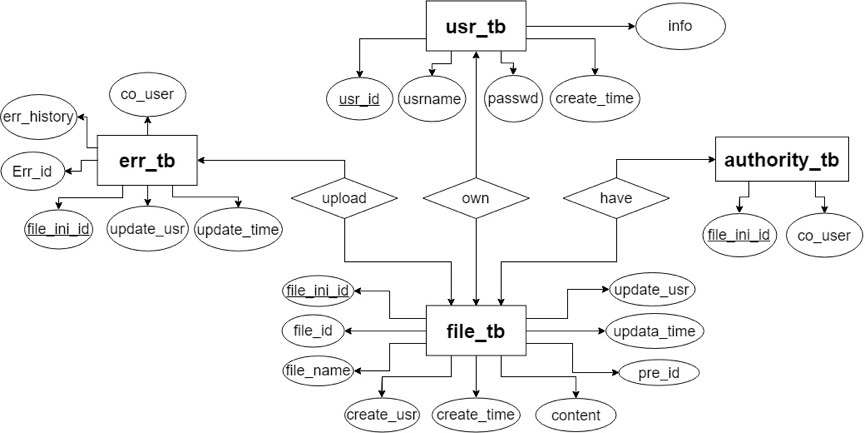
\includegraphics[width=.8\textwidth]{designdb.png} %图片文件的相对路径
  
  \label{png0} %此处的label相当于一个图片的专属标志,目的是方便上下文的引用
\end{figure}

\subsubsection{Transmission Protocol Design}
\noindent When choosing HTTP and HTTPS protocols, we originally wanted to choose HTTPS protocol. HTTPS protocol is a network protocol built by SSL+HTTP protocol for encrypted transmission and identity authentication. It is better than http protocol security and can better protect users’privacy. But considering that https needs to apply for a certificate, and there are very few free certificates. Finally, we still chose the HTTP protocol, which is relatively simple and convenient.

\subsubsection{UI Design}
\noindent After designing the first draft of the database, we have roughly identified some of the function keys for our UI interface design. The first is the welcome screen, there will be two options for registration and login. After logging in, you will be taken to the user's main page. You can see the user documentation and user information, in this page user can also upload and create new files. Click to enter the file page, the user can edit and rename the text, and the user can also add or delete the permissions of other users to this file. When there is a conflict in the uploaded file, there will be a file comparison page for the user to select the file they want to save.

\subsubsection{Some Other Details}
\noindent After completing the login screen, we first added the registration feature to join the new user. After the file modification function is completed, we have added the file renaming function for the file name that may need to be modified. Since we have considered that the file sync upload may overwrite the previous user's article, or if the user wants to view the old version and edit it, we have added the history section to view the old version. On this basis, we have adjusted the database again.



\section{Implementation}

\subsection{Significant Implementation Details}
\noindent After several months of unremitting efforts, we have tried many methods. From scratch, we have implemented several key functions of the original design step by step, and based on this, we have continuously improved and added some additional functions. We will introduce them separately from the web platform and the ios platform.

\subsubsection{Web Client}
\noindent User login interface introduction:
\begin{itemize}
    \item Registration function: When a user registers in this web page, he/she only needs to provide user-defined user name and password, after which the system will automatically assign a UID to the user. In the background system operation, the system background will automatically distinguish different users according to their UID.
    \item Login Function: In the process of implementing the login function, we extra use the channel encryption method to encrypt the user password.To be specific, we use the hash algorithm to ensure the security of the user. Because the hash function is unidirectional, once the user name and password are provided when the user registers, the system automatically assigns the UID background to distinguish the user according to the UID.
\end{itemize}

\noindent Home function introduction:
\begin{itemize}
    \item File Upload
    \item Display files with modified permissions
    \item File Sharing
    \item File Download
\end{itemize} 

\noindent Edit page function introduction
\begin{itemize}
    \item Content modification
%    \vspace{-0.3cm}
    \item File name modification: Logic: file is identified based on file id
    \item File creator can modify permissions.The historical version can be found and you can go back to the historical version for editing. Edit this version to the current version.
    \item Basic information about the file The person and time the file was last updated.
\end{itemize}

\noindent User Page Introduction



\subsection{Code Fragments and Explanation}
\subsubsection{Code Explanations of Desktop Client}
\noindent The code implementation of the registration function is shown in Fig.\ref{png1}. It first validates the user by requesting the \texttt{username} and the \texttt{password} from the user. The password must be 6-20 characters. After the validation, if the current user is not in the database, a new entry for the user will be created in the database user table with \texttt{create}. An ID is assigned to the user with \texttt{rand} function. After a successful registration, it will automatically jump to the login interface.

% The report must be at most 12,000 words or 35 pages (whichever is less)?超级爱你 我也爱你哦�� xin❤️xi��xin❤x❤️xi❤️❤️❤️nixnxin

\begin{figure}[H]
  \centering
  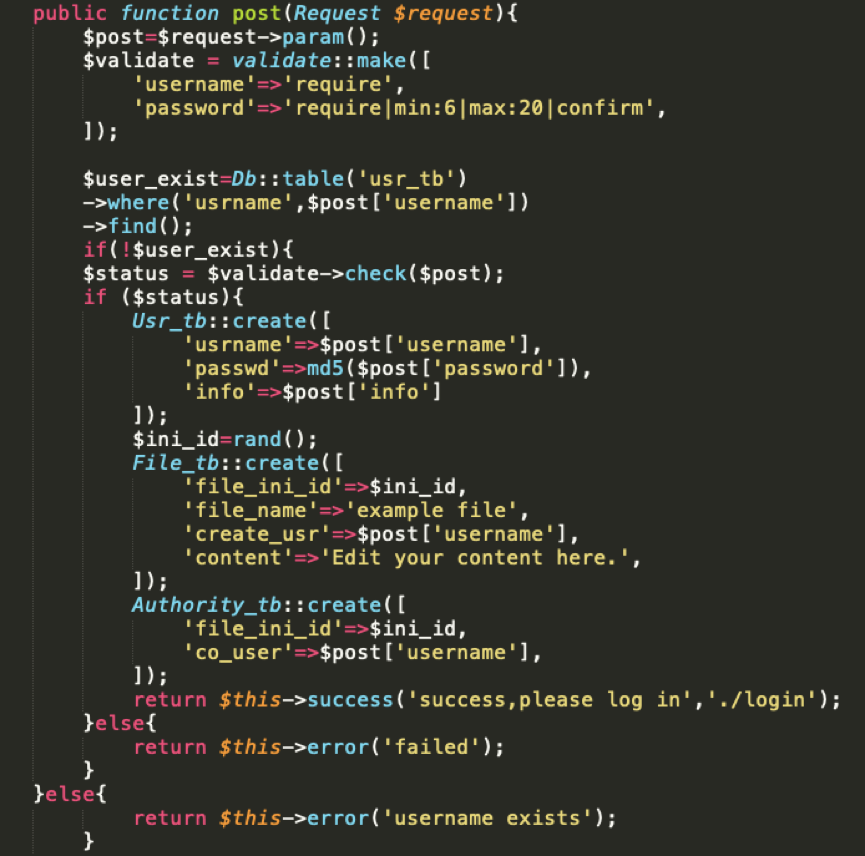
\includegraphics[width=.8\textwidth]{register.png} %图片文件的相对路径
  \caption{Code snippet of the registration function} %caption是图片的标题
  \label{png1} %此处的label相当于一个图片的专属标志,目的是方便上下文的引用
\end{figure}


\noindent The code implementation of the login function is shown in Fig.\ref{png2}. It first uses \texttt{IF} function to determine whether the user name received is the same as the username retrieved from the database. Then,the password is encrypted with \texttt{MD5} and the cipher text,which will be compared with the corresponding cipher in the session. Once the session values are equal, the user is verified to be successfully login and jumps automatically to the main web page(index.html).
\begin{figure}[H]
  \centering
  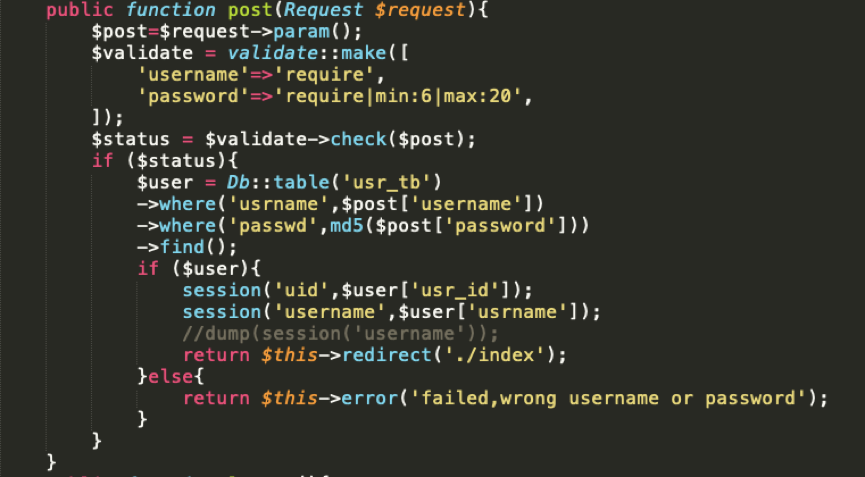
\includegraphics[width=.8\textwidth]{login.png} %图片文件的相对路径
  \caption{Code snippet of the login function} %caption是图片的标题
  \label{png2} %此处的label相当于一个图片的专属标志,目的是方便上下文的引用
\end{figure}

\noindent The code implementation of the file creation function is shown in Fig.\ref{png3}. It first generate and allocate file id by using \texttt{rand},then the database allocates space to this new file as well as update the permissions in the authority table.
\begin{figure}[H]
  \centering 
  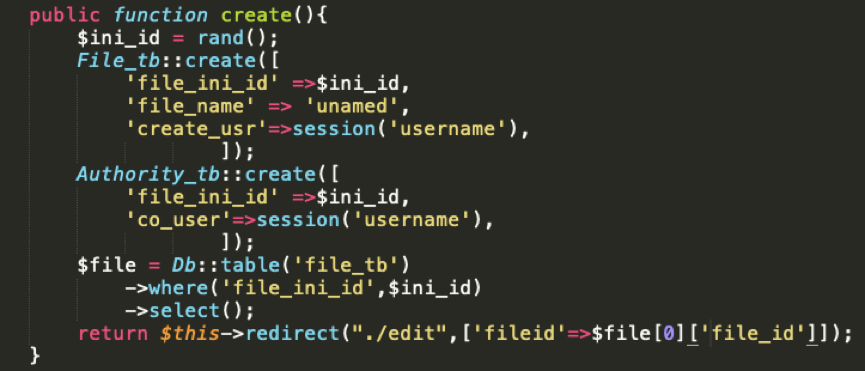
\includegraphics[width=.8\textwidth]{createfile.png} %图片文件的相对路径
  \caption{Code snippet of the file creation function} %caption是图片的标题
  \label{png3} %此处的label相当于一个图片的专属标志,目的是方便上下文的引用
\end{figure}



\noindent The code implementation of the file upload function is shown in Fig.\ref{png4}.The function of this code is to upload the existing local file to the database in the server.In detail,first and the most,it use the \texttt{IF}function to restrict the file type and size.After getting the local file path and extracting the contents of the file with \texttt{file\_get\_contents},it also randomly generates \texttt{file\_id}for the file.Finally, all the information relate to this file will be stored into the database.
\begin{figure}[H]
  \centering
  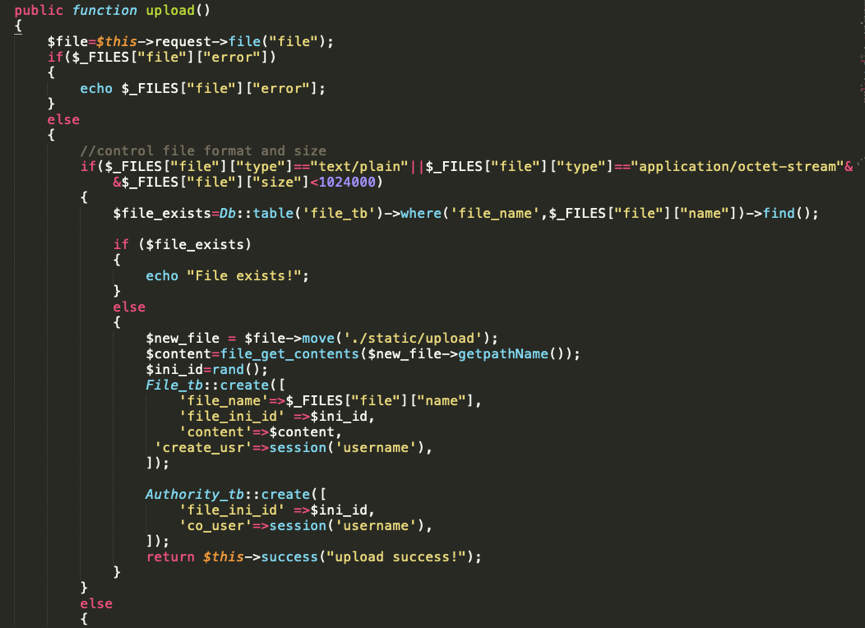
\includegraphics[width=.8\textwidth]{upnowfile.png} %图片文件的相对路径
  \caption{Code snippet of the file upload function} %caption是图片的标题
  \label{png4} %此处的label相当于一个图片的专属标志,目的是方便上下文的引用
\end{figure}


\noindent The code implementation of the file edit function is shown in Fig.\ref{png5}.In this edit interface, click \texttt{upload} to enter this function. Determine if there is a version error, if it does not exist, update the data to the database; if it exists, insert the data into the database and enter the compare page.

\begin{figure}[H]
  \centering
  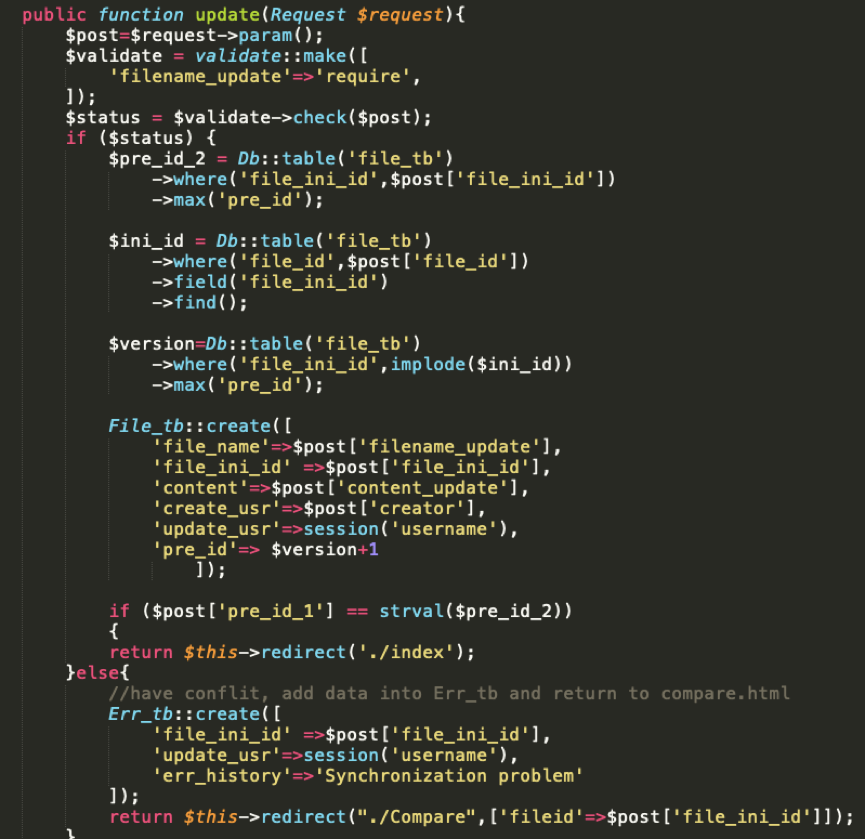
\includegraphics[width=.8\textwidth]{edit.png} %图片文件的相对路径
  \caption{Code snippet of the file edit function} %caption是图片的标题
  \label{png5} %此处的label相当于一个图片的专属标志,目的是方便上下文的引用
\end{figure}


\noindent The code implementation of adding coordinator function is shown in Fig.\ref{png6}.After determining whether there is a \texttt{username} to be added in \texttt{co\_user}, the system will operate differently depending on the particular case. If the coordinator already exists in database, it will not be added. If it does not exist, add this user into the permission table.
\begin{figure}[H]
  \centering
  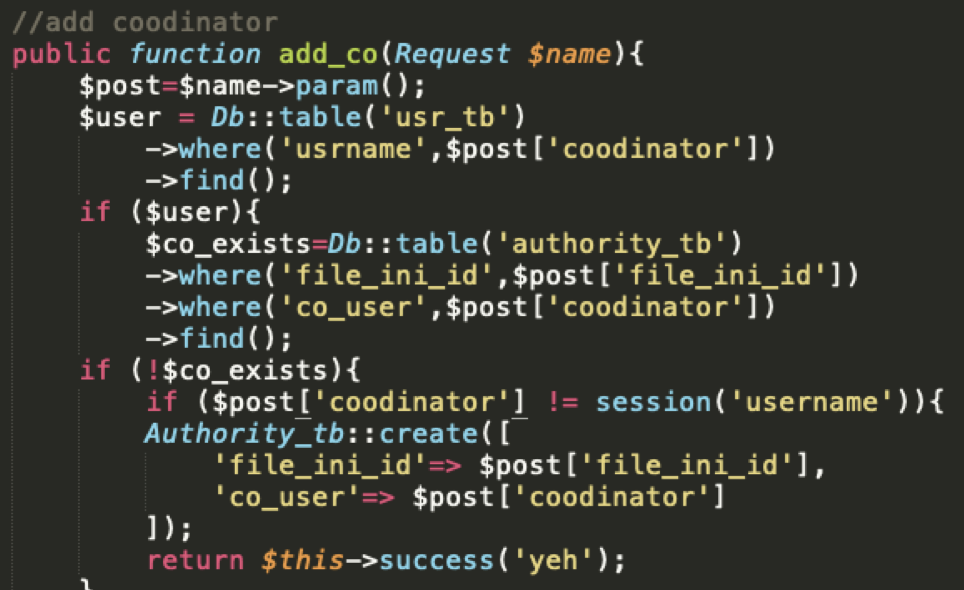
\includegraphics[width=.8\textwidth]{addco.png} %图片文件的相对路径
  \caption{Code snippet of adding coordinator function} %caption是图片的标题
  \label{png6} %此处的label相当于一个图片的专属标志,目的是方便上下文的引用
\end{figure}

\noindent The code implementation of Frontend modification permission function is shown in Fig.\ref{png7}.First, the if statement is used to determine that only the creator of the file will have the add and delete buttons. We can delete the edit authentication by their \texttt{username}.
\begin{figure}[H]
  \centering
  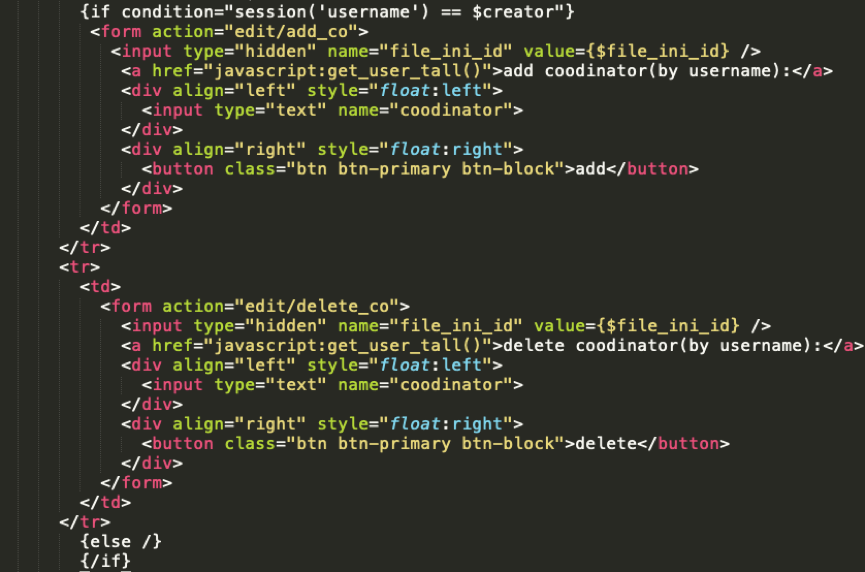
\includegraphics[width=.8\textwidth]{qianduan.png} %图片文件的相对路径
  \caption{} %caption是图片的标题
  \label{png7} %此处的label相当于一个图片的专属标志,目的是方便上下文的引用
\end{figure}



\noindent The code implementation of checking and returning to the historical version function is shown in Fig.\ref{png8}.
\begin{figure}[H]
  \centering
  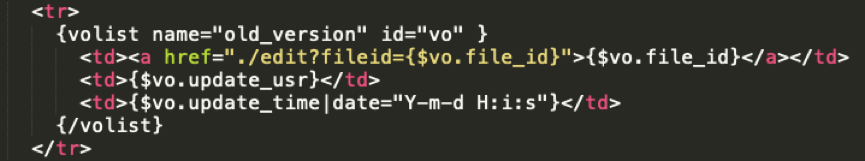
\includegraphics[width=.8\textwidth]{changeback.png} %图片文件的相对路径
  \caption{Code snippet of checking and returning to the historical version} %caption是图片的标题
  \label{png8} %此处的label相当于一个图片的专属标志,目的是方便上下文的引用
\end{figure}


\noindent The code implementation of checking and solving conflicts are shown separately in Fig.\ref{png9}.and Fig.\ref{png10}.This moment it have already encountered a conflict. According to the solution we designed, we need to construct a comparison page to compare the two conflicting documents together,and then, select the required version as the latest version according to the situation.
\noindent It gets the id of the file by using the \texttt{GET} command, then uses \texttt{fetch} to send the name and content of the two files to the compare page.
\noindent In the compare interface, the user can clearly see the contents of the two files and manually determine the version they want to keep, then they can choose to save this version of the file as the latest version.The code snippet in Fig.\ref{png10} is an example of saving the previous version of the file. After resetting the file\_id by \texttt{redirect}, it will automatically return to the index page.
\begin{figure}[H]
  \centering
  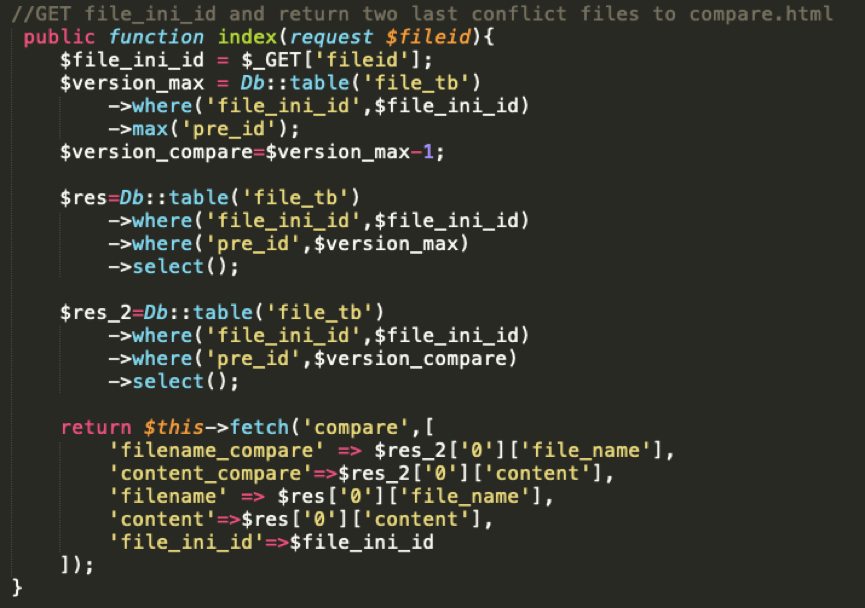
\includegraphics[width=.8\textwidth]{conflict.png}%图片文件的相对路径
  \caption{Code snippet of checking conflicts} %caption是图片的标题
  \label{png9} %此处的label相当于一个图片的专属标志,目的是方便上下文的引用
\end{figure}

\begin{figure}[H]
  \centering
  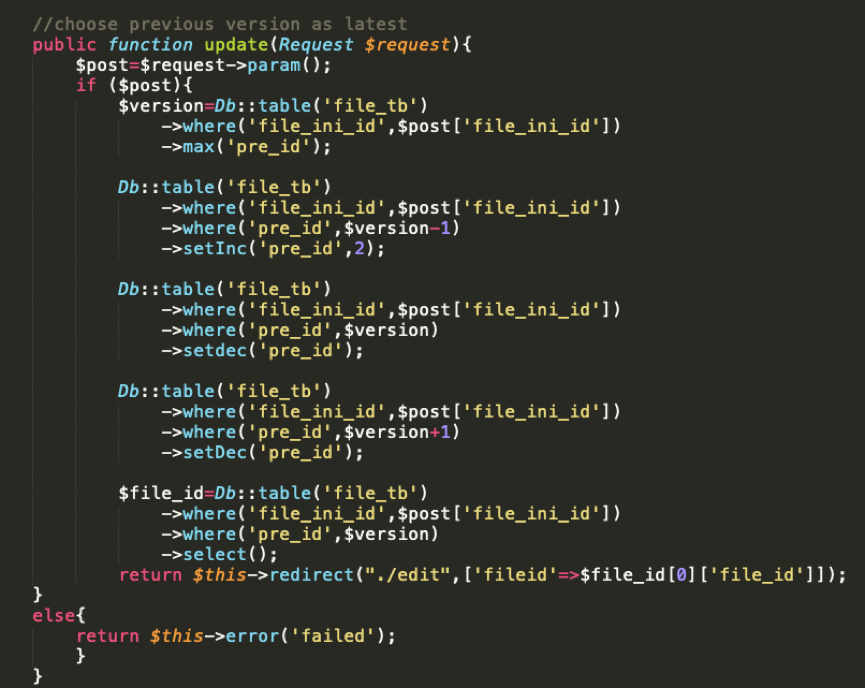
\includegraphics[width=.8\textwidth]{conflictsolve.png}%图片文件的相对路径
  \caption{Code snippet of saving the previous version} %caption是图片的标题
  \label{png10} %此处的label相当于一个图片的专属标志,目的是方便上下文的引用
\end{figure}




\subsubsection{IoS Mobile Client}

\subsection{Software Testing}
%关于ios客户端的unit testing


\noindent Our IoS mobile client uses the XCTest framework that comes with XCode. The word framework contains a class. All test classes inherit from this class. The name of this class is called XCTestCase. According to the regulations, the names of all test methods should start with the test and do not contain any parameters to ensure that these test methods are automatically executed when the test is run. In each test method, we call the function XCTAssert * to assert whether an operation was successful.

\section{Teamwork}
\noindent To facilitate our group work,we keep finding proper ways to solve potential difficulties and made specific plan to have meeting every week.In this section, we suppose to describe our teamwork in two aspects.

\subsection{Tools}
\noindent When it comes to what tools we choose to communicate with team members. We find face-to -face discussions is the most efficient way, followed by using Wechat and Git Hub.
\begin{itemize}
    \item Face-to-Face discussion: which are regarded by all the teammates as the most efficient way to solve problems and learn some knowledge together.
    \item Wechat: mainly used to share learning materials and make decision about meeting time and place. In addition, Wechat is a good tool we used to supplement the face-to-face communication because we could not spend all the time together.
    \item Git Hub: used to store main codes and report files and coordinate together with source code and commits.
\end{itemize}
\vspace{0.2cm}

\subsection{Main Processes}

\noindent First of all, our group holds one or two group discussions every week at the Waterloo campus library after we discuss the time that suitable for everyone in WeChat. Each meeting lasts about three hours.During the meeting time, we firstly make a simple report on the work done by everyone from the last meeting to the present, and then evaluate the completion rate of each person and improve the task allocation of each meeting, so that the work can be assigned according to each person's ability and the individual work will not be too much or too little. Then we will collect the unfinished tasks and determine the new tasks and goals we need to complete before the next meeting. We usually assign tasks through self-recommendation after discussing about all the upgrades.
 
 
 %However, there are some occasions that no one is interested in or good at these tasks. At this time, there is usually a teammate serves as an interim team leader to assign tasks. At the beginning, our face-to-face discussion was extremely inefficient. In two-hour meeting, because of mutual unfamiliarity and lack of clear purpose, everyone was gossiping and enjoying their self-study. After about three to four meetings, everyone became more active since we were familiar with each other. We were willing to speak out our own ideas even if we were not sure whether they were correct and we were willing to take the initiative to undertake tasks. When one of the member encounter difficulties, others will be enthusiastic to help him to find relevant materials and solutions. Our face-to-face discussions have therefore become more efficient and meaningful.
\vspace{0.2cm}


\noindent We created a conversation group in the WeChat application which is very helpful and efficient. Face-to-face meetings are not enough and we need dialogue anytime and anywhere. Everyone's work is interrelated, such as the front-end design and back-end response of the website, so the team members should communicate and negotiate frequently. In the group we will discuss the troubles we encountered when completing the assigned tasks after the meeting. At this time, teammates who are good at this field or experienced will provide solutions or suggestions. Thus, we don't have to wait until the next meeting but can quickly resolve problems without affecting the follow-up work.  In addition, we will also share relevant learning materials and insights in the WeChat group so that others can gain knowledge and make progress together.
On the use of GitHub, every member in our group have exposed to this tool, but only for simple upload and download operations. Therefore, in the initial establishment of the group, everyone created a new group, which was definitely a wrong operation. Later, we got familiar with the fork and pull request functions after reading the online information and watching the explaining video that recommended by lecturer. These two operations are very effective for our group work, By forking everyone got an individual project based on group project, which is essentially a new branch of the original project. we made improvements in our own personal projects, but they do not affect the code and structure of the group project. Then made a pull request based on Fork to the 'Captain', everyone in the group can see the changes directly and then comment on them. After everyone feels satisfied, the team leader will accept the improvements and merge them into the original project.
\vspace{0.2cm}

\noindent In the previous month, we discussed and recommended each person's work mainly through face-to-face meeting, so as you can see, our group interactions in GitHub were only pull request and directly merger in this period. However, the lecturer requested a more positive comment on each modification of the team projects, and we started using the comments function gradually.
\vspace{0.2cm}

\noindent In general, the coordination between each team members getting better and stronger when everyone was concern about their individual part at the beginning. Besides, the use of relevant tools are also more and more skilled, each member has a more profound understanding of aggregation and the process of teamwork.


\section{Evaluation}
\subsection{Advantages}
\begin{itemize}
    \item After later development and testing, we found that the MVC development model selected during the initial design process fits well with our project, Which explains that we have worked effectively during the initial resource browsing and filtering process, which finally help us to reduce the workload for subsequent development.
    \item Our code is written in a specification with a clear structure. The proportion of annotations is also appropriate, so it is very convenient for us to read and facilitate the reading and cooperation of other team members.
    \item In addition to special circumstances such as temporary scheduling, our team regularly organizes group meetings on Tuesdays and Fridays to discuss progress, learning and solving current problems. The members of the group are well-coordinated, and everyone has contributed to this group project and made their own contributions without disputes and irresponsible members.
    \item Before doing this project, the members of the group did not contact or use github. In the past few months, we gradually learned how to use github to save our own code and files from the blank state at the beginning.
    
\end{itemize}


\subsection{Disadvantages}
\begin{itemize}
    \item In the editing function of the file, at present we can only edit the .txt file, and the files in other formats have not been implemented yet.
    \item Although we have been learning how to use github, our technology is not very skilled when compared to the students who already have using experience. The frequency of using github of our group is not particularly high. Since we have more meetings per week, we also have other software to communicate within the group, so there is less balance between github interaction and other ways of communication.
\end{itemize}

\subsection{Differences from the Initial Idea}
\begin{itemize}
    \item Before we start doing this project, we intend to use the OT(Operation Transform) algorithm, which is a technology for supporting collaborative computing functions and applications to achieve collaboration.
    \item Later, in the process of studying this algorithm, we found that although this algorithm has advantages in operation conversion and processing collaborative editing, for our project, this algorithm is too complicated, and we want to achieve the core functions. It is not completely compatible. If we want to achieve simultaneous editing of files, the focus is not on OT-oriented design. That is, in design, the principle that is more conducive to the implementation of OT algorithm is the first, and the principle of reducing network transmission is second. In practice, it is necessary to have enough storage space to buffer the traffic difference between the two streams. The client OT must be a message that is bypassed, not a message processed by the database. This is more difficult for our system design and gpu requirements. Firstly, we searched for relevant materials about OT technology from the Internet since our team members are not familiar with this technology. There are various online instructions about OT algorithms using different computer languages such as Java, PHP, and Python.  But unfortunately, the tutorials using swift that our system gonna use are rare. In the process of trying to use OT, although it is easy to understand the principle of this technology, the actual operation is quite complicated. The reason why is that the OT algorithm is dependent on the order, and the different order will lead to different results. In addition, there will be some problem if the original file changed before the modification submit as the modification is based on the old version. Therefore, OT technology did not work well in our system, the bugs always appeared and we even cannot find solutions to solve them.So after finding a more simple and easy to implement method, we gave up the OT algorithm.
    
    \item We originally planned to use java to write mobile apps. But then we chose iOS to develop more commonly used swift. Swift supports both object-oriented programming and functional programming. Swift is more powerful than Java and more user-friendly. In addition, Xcode has a ready-made swift framework that makes our use and design easier.
\end{itemize}

\subsection{Detailed Evaluations}

\noindent Evaluations of the web front-end design and implementations:
\begin{itemize}
 
%songsong qianduan
    \item During the process of the development, we use the GIF image as the background of login page with a cute logo in order to make the webpage more vibrant, but the background is not coherent as it is hard to find a high-definition picture with coherent animation. when entering the index page, we originally prepared to use the uniform background color, but this is easy for users to feel boring, so we set different background images for each function page, and the pictures are all about nature, which makes the webpage more ornamental and eye-catching. For the choice of detail colors, we use the dark blue and gray that are generally accepted by the public.
    \item Except for the main function we have check user information, reset password and logout functions. Because the other three functions are auxiliary functions, we simplify the function bar and put it in the upper right corner. Thus, the user will see the main function page directly after login.
\end{itemize}


\noindent Evaluations of literature review and materials searching:
\begin{itemize}
    
%xiaoxue wenxian
    \item At the beginning, in order to make the progress of the post work progress, we found a lot of literature about file synchroniser. In the following group discussion, we classified the literature, which is roughly divided into front-end class, background class and function class. Then we learn the literature of the respective department responsible to determine the language of development, the algorithms needed, and the functions required by file synchroniser. The documents that are found later will be more practical, such as finding the iOS development language swift5, the main framework used by web development, , and the related literature about the MVC development model. The teammates who are looking for the literature are going to learn the specific functions to be implemented on the file synchroniser, such as the most basic editing and uploading, and constantly improve the functions and work with the coding students to communicate and learn related technologies together. In the final closing section, we will look at the literature to understand the meaning of this file synchroniser and its current status and prospects, and to understand the whole project more deeply.
\end{itemize}

\noindent Evaluations of the implementation of the main function:
\begin{itemize}
    \item As for how to solve the conflict problem, our group has gradually abandoned some algorithms and models that run the failure and do not support the development environment we choose in the process of continuous learning and practice. Eventually I thought of detecting conflicts by detecting the version number and comparison. This method is simple and easy to understand and is very fluent from a logical level. It is also convenient to convert to code implementation, and does not cause redundant work and complicated calculation comparison. It can be considered that the needs and ideas of the project have been completed and the main functions have been realized.
\end{itemize}

\noindent Evaluations of database design:
\begin{itemize}
    \item All entities and their properties of the database are meaningful. The naming of entities and attributes is also straightforward and easy understanding. Each value can be extracted for use successfully. The relationship between two entities is one-to-one, which reduces the complexity of extracting and importing data into the database.

    \item For database security, when the database is under attack and the data table is exposed, the attacker cannot see the user password that has been encrypted, which protects the privacy and security of the system user. But the file list is not encrypted, thus the attacker can read the file content directly and then easily tamper with or steal the information.

\end{itemize}

\noindent Evaluations of ThinkPHP usage:
\begin{itemize}
    \item We use PHP to write the server side of the web. In the beginning, we programmed it directly in PHP instead of using the framework. This method works well in the static web page, but we find it inconvenient when we want to connect it to the database or add links to each other. After discussion, we re-planned the architecture of the website and determined to use the framework of ThinkPHP, because of its perfect integrated configuration which can simplify the step of the database connection.
    \item Although this experience took a lot of time and effort, timely re-planning made our project smooth and even better. Besides, our team members also have a better understanding of PHP and ThinkPHP in the process.

\end{itemize}

\noindent Evaluations of swift usage:
\begin{itemize}
    \item The swift language is one of the common languages developed by iOS. It is fast, secure and modern. Before the project started, we didn't have any knowledge of the language. After this period of study, we gradually understood how to use the swift language for development. And before our project was completed, swift was updated with a new version. The updated features were somewhat different from the previous ones, and we were able to update and improve in time.
\end{itemize}


\subsection{Future Work}

\noindent The future work contains five sides:

\begin{itemize}
    \item The function downloading is needed when we only have uploading and sharing currently. To implement this function, there are two typical ways. Firstly, we think about the standard URL download which is embedding an URL hyperlink in the web page and then downloading using a standard HTTP GET request. However, the drawback of this method is that the path of the file is completely exposed, which leads to a low security and privacy of the website. The second method is to submit the form, submitting the parameters to the server-side dynamic script by using POST request, and then the server-side script returns the output binary stream to the browser for download. This downloading method is not only available for the specific files on server but also for the data that dynamically generated by server. We will experiment with both methods and choose the one that works best.
    \item Various privilege will be set. Now, the users can directly view and modify the file when the file creator add them. In the future, we will divide permissions into read, write, and operation which contains deleting, downloading and sharing file. The owner of a file will have both these three permissions on the file initially. Besides, only the owner can edit the privilege of the file and he/she can let other users to only read, only operate or do nothing on the specific file as they want. To achieve this function, we will need to build the privilege table for each file, and the table should be automatically generated and deleted with the file.
    \item At present our project can only support the operation on the file that browser can open directly like txt. We will improve the system to handle different types of files like excel and pdf. 
    \item Our project is based on local database without server to save time and money as the lease of the server is expensive, and the connection to the server is complicated, which involves licensing, installation, maintenance, support, and patching associated with the operating system. However, Serverless computing is not suitable for workloads with high computing performance requirements due to the limitations on resources, and there are many application components in the serverless architecture, so the system is also in high risk to be attacked. Thus, in the future work, we will try to connect our system to the server.
    \item The file table in the database will be encrypted as it can be read directly and malicious tamped when being attacked. We have encrypted the user password with the hash algorithm, but the hash algorithm is irreversible, so we are going to find other encryption algorithms to encrypt the file content. Most of the common encryption methods are one-way and irreversible, we consider to encrypt the content during the transmission process, which means we are going to use protocol encryption like HTTPS.

\end{itemize}







\section{Peer Assessment}
\noindent After unanimous consent of the members of the group, we use a simple table to show the distribution of the scores of members in our group.


    
\begin{center}

\begin{table}[H]
\centering
\begin{tabular}{ccll}
\rowcolor[HTML]{FD6864} 
{\color[HTML]{333333} Name} & {\color[HTML]{333333} Grades} \\ \hline
Ji,Dongang                  & 18                            \\ \hline
Peng,Xiaoyue                & 18                            \\ \hline
Bai,Xiaoxue                 & 16                            \\ \hline
Zhan,Xiao                   & 16                            \\ \hline
Yu,Ying                     & 16                            \\ \hline
Song,Yingdi                 & 16                            \\ \hline
\end{tabular}
\end{table}
    
\end{center}



\newpage
% \printbibliography
% \section{reference}
% \begin{thebibliography}{9}

% \bibitem{adams1995hitchhiker}

% \end{thebibliography}

\bibliographystyle{plain}
\bibliography{references}


\end{document}




